\documentclass[a4paper]{beamer}
%
% Thesis Defense Presentation
%
\usepackage[utf8]{inputenc}
\usepackage{color}
\usepackage{tikz}
\usetikzlibrary{shapes.geometric, arrows.meta, positioning}
\usetheme{Frankfurt}
\useinnertheme{circles}
\usepackage[english]{babel}
\usefonttheme{professionalfonts}
%
\def\uv#1{\char92\relax #1\char34\relax}
%%%%%%%%%%%%%%%%%%%%%%%%%%%%%%%%%%%%%%%%%%%%%%%%%%%%%%%%%%%%%%%%%%
\newcommand\FirstName{Bilguudei}
\newcommand\FirstNameAbbreviated{B}
\newcommand\LastName{Baljinnyam}
\newcommand\Email{baljibil@fit.cvut.cz}
\newcommand\DissertationTitle{Rty: A Statically Typed R-like Language\\Targeting WebAssembly}
\newcommand\Department{Department of Theoretical Computer Science}
\newcommand\Faculty{Faculty of Information Technology}
\newcommand\University{Czech Technical University in Prague}
\newcommand\FacultyAndUniversityAbbr{FIT CTU}
%%%%%%%%%%%%%%%%%%%%%%%%%%%%%%%%%%%%%%%%%%%%%%%%%%%%%%%%%%%%%%%%%%
\subject{Programming Languages and Compilers}
\author[\FirstNameAbbreviated. \LastName]{\FirstName{} \LastName}
\title{\DissertationTitle}
\titlegraphic{\includegraphics[width=1.5cm]{pic/LogoCVUT.pdf}}
\institute[\FacultyAndUniversityAbbr]{\Department\\ \Faculty\\ \University}
\date{\today}
%
\begin{document}
\begin{frame}
\titlepage
\end{frame}

\section{Outline}
\subsection*{Outline}
\begin{frame}
\frametitle{Outline}
\tableofcontents
\end{frame}

\section{Introduction}
\subsection*{Introduction}
\begin{frame}
\frametitle{Motivation}
\begin{itemize}
\item \textbf{R language}: Popular for data science and statistics
\begin{itemize}
    \item Dynamic typing, interpreted execution
    \item Performance bottlenecks for production workloads
\end{itemize}
\vspace*{0.3cm}
\item \textbf{WebAssembly}: High-performance portable compilation target
\begin{itemize}
    \item Near-native speed in browsers and servers
    \item GC proposal enables high-level language features
\end{itemize}
\vspace*{0.3cm}
\item \textbf{Problem}: No statically typed R-like language for WASM
\begin{itemize}
    \item Type safety for production pipelines
    \item Performance through ahead-of-time compilation
\end{itemize}
\end{itemize}
\end{frame}

\begin{frame}[fragile]
\frametitle{Rty Language Overview}
\begin{itemize}
\item R-compatible syntax with optional type annotations
\item Statically typed with type inference
\item First-class functions with closures
\item Lexical scoping with superassignment (\texttt{<<-})
\item Compiles to WebAssembly
\end{itemize}

\vspace*{0.3cm}
\begin{exampleblock}{Example Code}
{\small
\begin{verbatim}
add <- function(a: int, b: int): int {
  return(a + b)
}

apply <- function(f: int -> int, x: int): int {
  return(f(x))
}
\end{verbatim}
}
\end{exampleblock}
\end{frame}

\begin{frame}
\frametitle{Contributions of the Thesis}
\begin{enumerate}
\item \textbf{Type System \& Formal Semantics}
\begin{itemize}
    \item Sound static type system with polymorphic vectors
    \item Structural typing for first-class functions
    \item Formalized operational semantics
\end{itemize}
\vspace*{.3cm}
\item \textbf{Novel Compilation Techniques}
\begin{itemize}
    \item WASM GC subtyping for closures
    \item Reference cells for mutable captures
    \item Multi-pass IR transformation
\end{itemize}
\vspace*{.3cm}
\item \textbf{Working Compiler Implementation}
\begin{itemize}
    \item $\sim$8,500 lines of Rust
    \item Comprehensive test suite
    \item Performance evaluation: 2.6--3.2$\times$ speedup over R
\end{itemize}
\end{enumerate}
\end{frame}

\section{Language Design}
\subsection*{Type System}
\begin{frame}
\frametitle{Type System}
\begin{block}{Types}
$\tau ::= \texttt{int} \mid \texttt{double} \mid \texttt{string} \mid \texttt{logical} \mid \texttt{vector}\langle\tau\rangle \mid \tau_1, \ldots, \tau_n \to \tau$
\end{block}

\begin{block}{Key Typing Rules}
\begin{itemize}
\item \textbf{Function types}: $\Gamma, x_1:\tau_1, \ldots, x_n:\tau_n \vdash e : \tau \Rightarrow \Gamma \vdash \texttt{function}(x_1:\tau_1, \ldots, x_n:\tau_n):\tau\{e\} : \tau_1,\ldots,\tau_n \to \tau$
\item \textbf{Vector operations}: Homogeneous element types
\item \textbf{Numeric promotion}: $\texttt{int} <: \texttt{double}$
\item \textbf{Superassignment}: Modifies parent scope bindings
\end{itemize}
\end{block}

\begin{alertblock}{Type Safety}
Informal soundness argument: Progress + Preservation properties
\end{alertblock}
\end{frame}

\section{Compiler Architecture}
\subsection*{Pipeline}
\begin{frame}
\frametitle{Compilation Pipeline}
\begin{center}
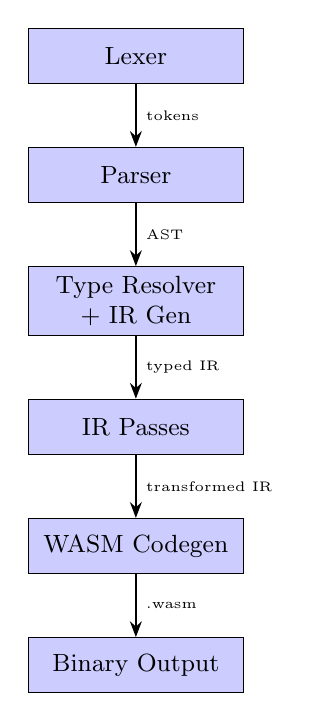
\begin{tikzpicture}[
    node distance=0.8cm,
    box/.style={rectangle, draw, fill=blue!20, text width=2.5cm, align=center, minimum height=0.7cm, font=\small},
    arrow/.style={-{Stealth[length=2mm]}, thick}
]
\node[box] (lex) {Lexer};
\node[box, below=of lex] (parse) {Parser};
\node[box, below=of parse] (ir) {Type Resolver\\+ IR Gen};
\node[box, below=of ir] (passes) {IR Passes};
\node[box, below=of passes] (codegen) {WASM Codegen};
\node[box, below=of codegen] (output) {Binary Output};

\draw[arrow] (lex) -- node[right, font=\tiny] {tokens} (parse);
\draw[arrow] (parse) -- node[right, font=\tiny] {AST} (ir);
\draw[arrow] (ir) -- node[right, font=\tiny] {typed IR} (passes);
\draw[arrow] (passes) -- node[right, font=\tiny] {transformed IR} (codegen);
\draw[arrow] (codegen) -- node[right, font=\tiny] {.wasm} (output);
\end{tikzpicture}
\end{center}

\begin{itemize}
\item \textbf{IR Passes}: Variable collection, capture analysis, function flattening
\item \textbf{Output}: Binary WASM + text WAT format
\end{itemize}
\end{frame}

\subsection*{Closure Compilation}
\begin{frame}
\frametitle{Closure Compilation with WASM GC}
\framesubtitle{Novel Use of Structural Subtyping}

\begin{block}{Challenge}
How to compile closures with captured variables to WebAssembly?
\end{block}

\begin{exampleblock}{Solution: Environment Structs with Subtyping}
\begin{itemize}
\item \textbf{Base type}: \texttt{(struct (field \$func\_ptr (ref func)))}
\item \textbf{Concrete type}: Subtype with captured variable fields
\item Function pointer + captured variables in single struct
\item WASM validates downcast at runtime
\end{itemize}
\end{exampleblock}

\begin{alertblock}{Key Advantage}
\begin{itemize}
\item Type-safe closure representation
\item No function tables needed (uses \texttt{call\_ref})
\item Efficient with WASM GC automatic memory management
\end{itemize}
\end{alertblock}
\end{frame}

\begin{frame}[fragile]
\frametitle{Reference Cells for Mutable Captures}
\framesubtitle{Implementing R's Superassignment}

\begin{block}{R Superassignment (\texttt{<<-})}
Modifies variable in parent scope --- requires mutable sharing
\end{block}

\begin{columns}
\begin{column}{0.5\textwidth}
\begin{exampleblock}{R Code}
{\tiny
\begin{verbatim}
counter <- function() {
  x: int <- 0
  inc <- function() {
    x <<- x + 1
  }
  return(inc)
}
\end{verbatim}
}
\end{exampleblock}
\end{column}
\begin{column}{0.5\textwidth}
\begin{alertblock}{Strategy}
{\small
\begin{itemize}
\item Wrap \texttt{x} in reference cell struct
\item Both closures share same cell
\item Read: \texttt{struct.get}
\item Write: \texttt{struct.set}
\end{itemize}
}
\end{alertblock}
\end{column}
\end{columns}

\vspace*{0.2cm}
\textbf{Result}: Statically typed mutable captures without escape analysis
\end{frame}

\section{Evaluation}
\subsection*{Correctness}
\begin{frame}
\frametitle{Correctness \& Testing}
\begin{itemize}
\item \textbf{Test Suite Coverage}:
\begin{itemize}
    \item Unit tests: Lexer, parser, type resolution, first-class functions
    \item Integration tests: WASM generation, end-to-end compilation
    \item 40+ validation programs in \texttt{data/} directory
\end{itemize}

\vspace*{0.3cm}
\item \textbf{Cross-validation}:
\begin{itemize}
    \item Compare Rty output vs. native R interpreter
    \item Type erasure ensures semantic equivalence
    \item Differential testing validates compiler correctness
\end{itemize}

\vspace*{0.3cm}
\item \textbf{Type Safety}:
\begin{itemize}
    \item Informal soundness argument (Progress + Preservation)
    \item WASM validation confirms type correctness
    \item All generated code passes \texttt{wasmtime --validate}
\end{itemize}
\end{itemize}
\end{frame}

\subsection*{Performance}
\begin{frame}
\frametitle{Performance Results}
\framesubtitle{Apple M1, R 4.3.1, Wasmtime 16.0.0}

\begin{table}
\centering
\small
\begin{tabular}{lrrr}
\hline
\textbf{Benchmark} & \textbf{R (ms)} & \textbf{Rty (ms)} & \textbf{Speedup} \\
\hline
Integer sum (10k) & 155 & 57 & \textcolor{green}{\textbf{2.71$\times$}} \\
Vector addition (10k) & 155 & 57 & \textcolor{green}{\textbf{2.71$\times$}} \\
Fibonacci(25) & 185 & 57 & \textcolor{green}{\textbf{3.24$\times$}} \\
Nested loops (1M) & 183 & 65 & \textcolor{green}{\textbf{2.81$\times$}} \\
Closure creation (10k) & 154 & 59 & \textcolor{green}{\textbf{2.61$\times$}} \\
\hline
\end{tabular}
\end{table}

\begin{block}{Analysis}
\begin{itemize}
\item Consistent 2.6--3.2$\times$ speedup over interpreted R
\item Static types enable optimization and inlining
\item WASM GC overhead is minimal
\end{itemize}
\end{block}

\begin{exampleblock}{Compilation Time}
Fast enough for interactive workflows: 69--74ms per file
\end{exampleblock}
\end{frame}

\section{Summary}
\subsection*{Summary}
\begin{frame}
\frametitle{Summary}
\begin{enumerate}
\item \textbf{Demonstrated feasibility} of statically typed R-like language
\begin{itemize}
    \item Core R features amenable to static typing
    \item Type safety without sacrificing expressiveness
\end{itemize}

\vspace*{0.2cm}
\item \textbf{Novel compilation techniques} for WebAssembly
\begin{itemize}
    \item WASM GC subtyping for efficient closures
    \item Reference cells for mutable captures
\end{itemize}

\vspace*{0.2cm}
\item \textbf{Significant performance improvements}
\begin{itemize}
    \item 2.6--3.2$\times$ speedup over interpreted R
    \item Enables deployment in browsers and edge devices
\end{itemize}

\vspace*{0.2cm}
\item \textbf{Foundation for future work}
\begin{itemize}
    \item Clean architecture: $\sim$8,500 lines Rust
    \item Comprehensive test suite
    \item Extensible design for additional features
\end{itemize}
\end{enumerate}
\end{frame}

\subsection*{Future Work}
\begin{frame}
\frametitle{Future Work}
\begin{block}{Short-term}
\begin{itemize}
\item Expand type system (structs, union types, type aliases)
\item More statistical built-ins (mean, sd, cor, matrix ops)
\item Optimization passes (constant folding, inlining, DCE)
\item Better error messages with source locations
\end{itemize}
\end{block}

\begin{block}{Medium-term}
\begin{itemize}
\item SIMD vectorization using WASM SIMD proposal
\item FFI to JavaScript/WASI for I/O and libraries
\item Generic functions with type parameters
\item Pattern matching and destructuring
\end{itemize}
\end{block}

\begin{block}{Long-term}
\begin{itemize}
\item Interactive REPL with incremental compilation
\item Package system and dependency management
\item Native backend (LLVM or Cranelift)
\end{itemize}
\end{block}
\end{frame}

\subsection*{Contributions}
\begin{frame}
\frametitle{Contributions of the Thesis}
\textbf{Main contributions:}
\bigskip
\begin{enumerate}
\item \textbf{Formal Type System}
\begin{itemize}
    \item Sound static type system for R-like language
    \item First-class functions with structural typing
    \item Formalized operational semantics
\end{itemize}
\vspace*{.3cm}
\item \textbf{Novel Compilation Techniques}
\begin{itemize}
    \item WASM GC subtyping for closures
    \item Reference cells for mutable captures
    \item Multi-pass IR transformation architecture
\end{itemize}
\vspace*{.3cm}
\item \textbf{Working Implementation}
\begin{itemize}
    \item Complete compiler: lexer, parser, type checker, codegen
    \item Comprehensive test suite and validation
    \item Demonstrated 2.6--3.2$\times$ performance improvement
\end{itemize}
\end{enumerate}
\end{frame}

\section*{Discussion}
\subsection*{Discussion}
\begin{frame}
\begin{center}
\vspace*{1cm}
{\bf Thank you for your attention!}\\
\vspace*{1cm}
{\large Questions?}
\vspace*{1.5cm}

{\bf\Large \FirstName{} \LastName{}}\\
{\tt \Email}\\
\vspace*{0.5cm}
{\small \Department}\\
{\small \Faculty}\\
{\small \University}
\end{center}
\vfill
{\tiny \textbf{Acknowledgement:} This research was conducted at the Faculty of Information Technology, Czech Technical University in Prague.}
\end{frame}

%
\appendix
\section{Backup Slides}
\subsection{Type System Details}
\begin{frame}
\frametitle{Type System: Core Rules}
\begin{block}{Variable and Literals}
$\frac{x:\tau \in \Gamma}{\Gamma \vdash x : \tau}$ \quad
$\frac{}{\Gamma \vdash n : \texttt{int}}$ \quad
$\frac{}{\Gamma \vdash d : \texttt{double}}$
\end{block}

\begin{block}{Function Application}
$\frac{\Gamma \vdash e_1 : \tau_1,\ldots,\tau_n \to \tau \quad \Gamma \vdash e_2 : \tau_1 \quad \cdots \quad \Gamma \vdash e_{n+1} : \tau_n}{\Gamma \vdash e_1(e_2, \ldots, e_{n+1}) : \tau}$
\end{block}

\begin{block}{Vector Construction}
$\frac{\Gamma \vdash e_1 : \tau \quad \cdots \quad \Gamma \vdash e_n : \tau}{\Gamma \vdash \texttt{c}(e_1, \ldots, e_n) : \texttt{vector}\langle\tau\rangle}$
\end{block}
\end{frame}

\subsection{Implementation Statistics}
\begin{frame}
\frametitle{Implementation Statistics}
\begin{block}{Codebase}
\begin{itemize}
\item Total: $\sim$8,500 lines of Rust
\item Core compiler: $\sim$6,000 lines
\item Tests: $\sim$2,500 lines
\end{itemize}
\end{block}

\begin{block}{Module Organization}
\begin{itemize}
\item \texttt{src/types/}: Cross-cutting type definitions
\item \texttt{src/lexer.rs}: Tokenization (350 lines)
\item \texttt{src/parser/}: Parsing (1,200 lines)
\item \texttt{src/ir/}: Type resolution and passes (2,000 lines)
\item \texttt{src/backend/}: Code generation (2,500 lines)
\item \texttt{src/driver/}: I/O orchestration (500 lines)
\end{itemize}
\end{block}

\begin{block}{Dependencies}
\texttt{wasm-encoder}, \texttt{wasmprinter}, \texttt{wasmtime}
\end{block}
\end{frame}

\end{document}
